\element{transmetteurs}{
\begin{question}{tr 01}
Soit le schéma suivant. Déterminer $\dfrac{\omega_{20}}{\omega_{10}}$.
\begin{center}
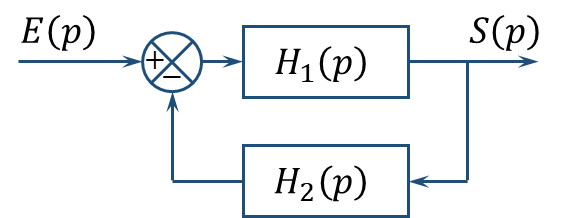
\includegraphics[width=5cm]{fig_01}
\end{center}
\begin{multicols}{4}
	\begin{reponses}	
	\mauvaise{$-\dfrac{Z_2}{Z_1}$}
	\mauvaise{$\dfrac{Z_2}{Z_1}$}
	\bonne{$-\dfrac{Z_1}{Z_2}$}
	\mauvaise{$\dfrac{Z_1}{Z_2}$}
	\end{reponses}
\end{multicols}
\end{question}\\}

\element{transmetteurs}{
\begin{question}{tr 02}
Soit le schéma suivant. Déterminer $\dfrac{\omega_{10}}{\omega_{20}}$.
\begin{center}
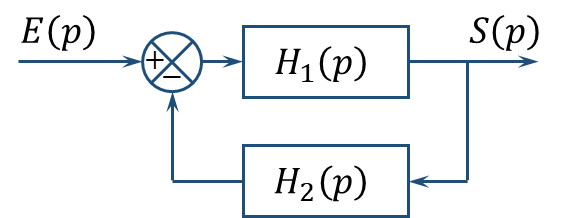
\includegraphics[width=5cm]{fig_01}
\end{center}
\begin{multicols}{4}
	\begin{reponses}	
	\bonne{$-\dfrac{Z_2}{Z_1}$}
	\mauvaise{$\dfrac{Z_2}{Z_1}$}
	\mauvaise{$-\dfrac{Z_1}{Z_2}$}
	\mauvaise{$\dfrac{Z_1}{Z_2}$}
	\end{reponses}
\end{multicols}
\end{question}\\}

\element{transmetteurs}{
\begin{question}{tr 03}
Soit le schéma suivant. Déterminer $\dfrac{\omega_{20}}{\omega_{10}}$.
\begin{center}
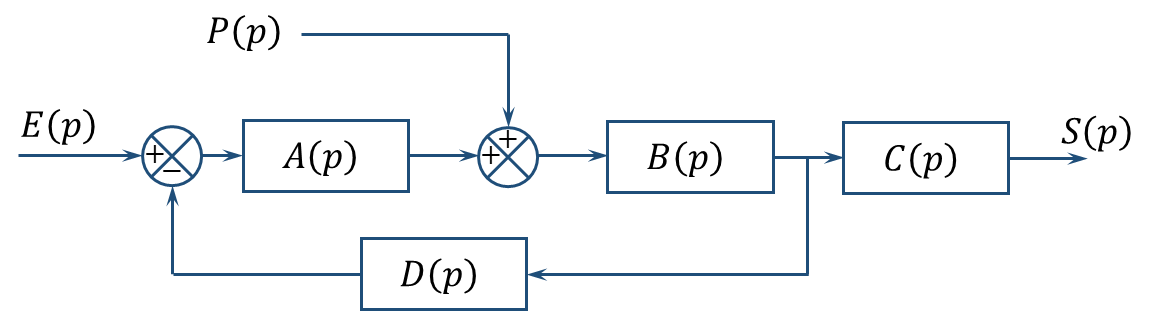
\includegraphics[width=5cm]{fig_02}
\end{center}
\begin{multicols}{4}
	\begin{reponses}	
	\mauvaise{$\dfrac{Z_2}{Z_1}$}
	\mauvaise{$-\dfrac{Z_2}{Z_1}$}
	\mauvaise{$-\dfrac{Z_1}{Z_2}$}
	\bonne{$\dfrac{Z_1}{Z_2}$}
	\end{reponses}
\end{multicols}
\end{question}\\}

\element{transmetteurs}{
\begin{question}{tr 04}
Soit le schéma suivant. Déterminer $\dfrac{\omega_{10}}{\omega_{20}}$.
\begin{center}
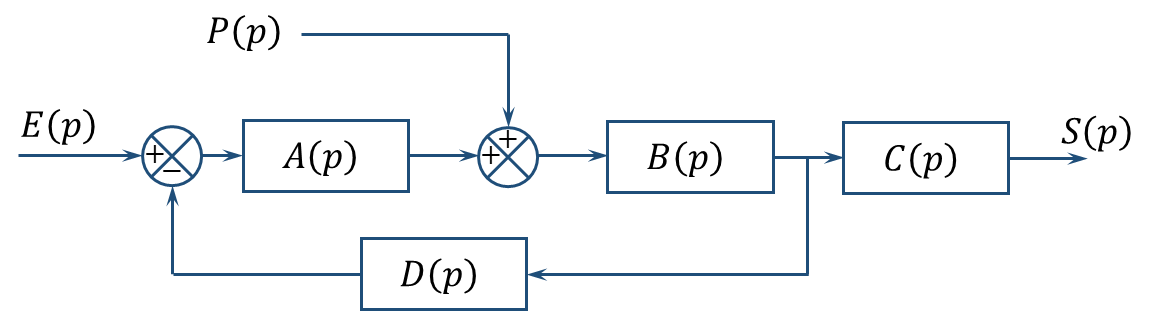
\includegraphics[width=5cm]{fig_02}
\end{center}
\begin{multicols}{4}
	\begin{reponses}	
	\bonne{$-\dfrac{Z_2}{Z_1}$}
	\mauvaise{$\dfrac{Z_2}{Z_1}$}
	\mauvaise{$\dfrac{Z_1}{Z_2}$}
	\mauvaise{$-\dfrac{Z_1}{Z_2}$}
	\end{reponses}
\end{multicols}
\end{question}\\}


\element{transmetteurs}{
\begin{question}{tr 05}
Soit le schéma suivant. Déterminer $\dfrac{\omega_{20}}{\omega_{10}}$.
\begin{center}
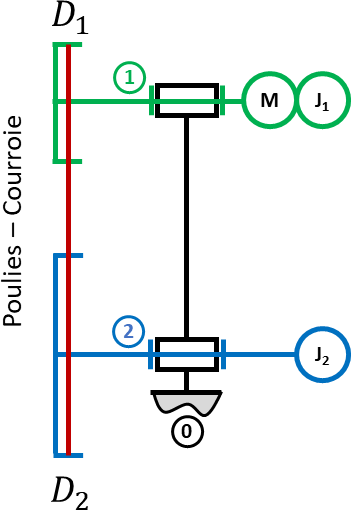
\includegraphics[width=5cm]{fig_03}
\end{center}
\begin{multicols}{4}
	\begin{reponses}	
	\mauvaise{$\dfrac{D_2}{D_1}$}
	\mauvaise{$-\dfrac{D_2}{D_1}$}
	\mauvaise{$-\dfrac{D_1}{D_2}$}
	\bonne{$\dfrac{D_1}{D_2}$}
	\end{reponses}
\end{multicols}
\end{question}\\}

\element{transmetteurs}{
\begin{question}{tr 06}
Soit le schéma suivant. Déterminer $\dfrac{\omega_{10}}{\omega_{20}}$.
\begin{center}
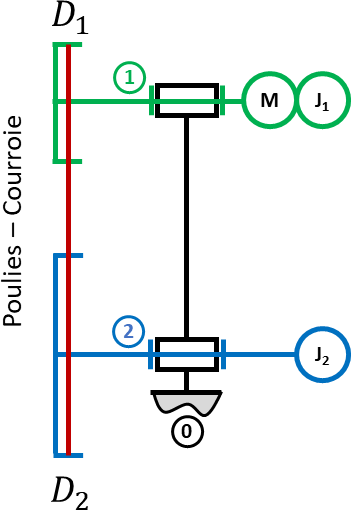
\includegraphics[width=5cm]{fig_03}
\end{center}
\begin{multicols}{4}
	\begin{reponses}	
	\mauvaise{$-\dfrac{D_2}{D_1}$}
	\bonne{$\dfrac{D_2}{D_1}$}
	\mauvaise{$\dfrac{D_1}{D_2}$}
	\mauvaise{$-\dfrac{D_1}{D_2}$}
	\end{reponses}
\end{multicols}
\end{question}\\}



\element{transmetteurs}{
\begin{question}{tr 07}
On note $v$ la vitesse de la charge $M$ selon la direction verticale. Exprimer $v$ en fonction de 
$\omega_{10}$ (en valeur absolue).
\begin{center}
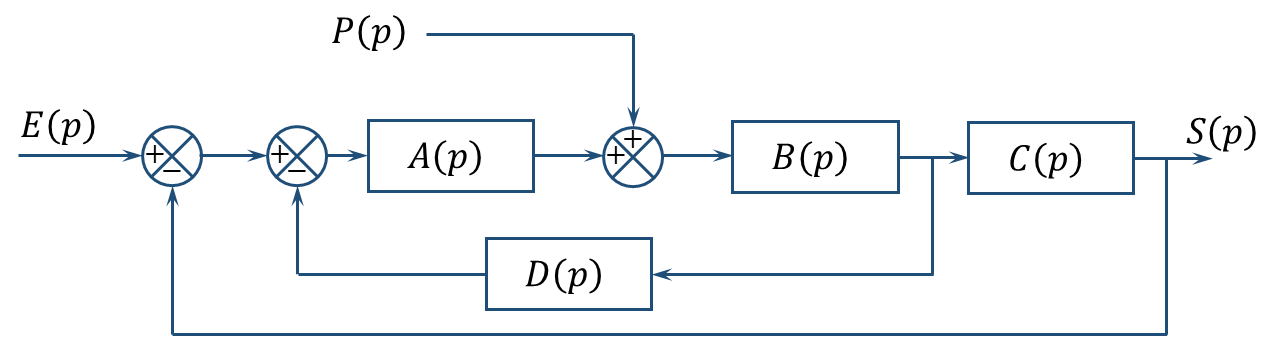
\includegraphics[width=5cm]{fig_04}
\end{center}
\begin{multicols}{4}
	\begin{reponses}	
	\mauvaise{$v = \dfrac{D_2 }{D_1 D_3} \omega_{10}$}
	\mauvaise{$v = \dfrac{D_2 D_3 }{D_1}\omega_{10}$}
	\mauvaise{$v = \dfrac{D_1 D_3 }{D_2} \omega_{10}$}
	\bonne{$v = \dfrac{D_1 D_3}{2 D_2 } \omega_{10}$}
	\end{reponses}
\end{multicols}
\end{question}\\}


\element{transmetteurs}{
\begin{question}{tr 08}
On note $v$ la vitesse de la charge $M$ selon la direction horizontale. Exprimer $v$ en fonction de
$\omega_{10}$ (en valeur absolue). On note $m$ le module des roues dentées.
\begin{center}
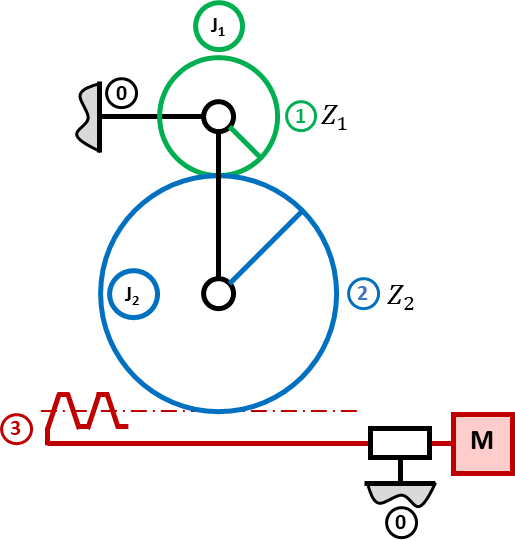
\includegraphics[width=5cm]{fig_05}
\end{center}
\begin{multicols}{4}
	\begin{reponses}	
	\mauvaise{$v = \dfrac{Z_2}{Z_1 } \omega_{10}$}
	\mauvaise{$v = \dfrac{m Z_2}{Z_1 } \omega_{10}$}
	\mauvaise{$v = \dfrac{Z_2^2}{2 Z_1 } \omega_{10}$}
	\bonne{$v = \dfrac{m Z_2}{2 Z_1 Z_2} \omega_{10}$}
	\end{reponses}
\end{multicols}
\end{question}\\}

\element{transmetteurs}{
\begin{question}{tr 09}
Exprimer $\omega_{10}$ en fonction de $\omega_{30}$ (en valeur absolue). 
\begin{center}
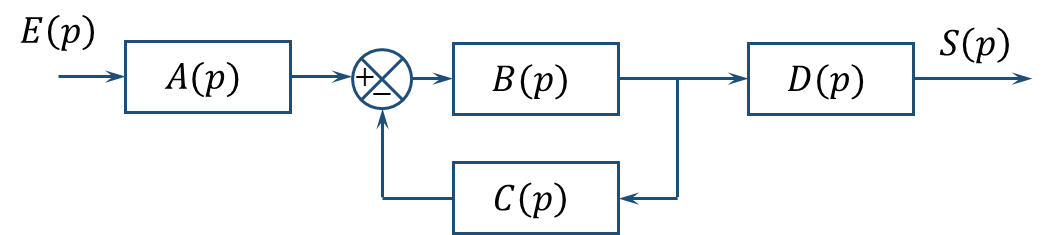
\includegraphics[width=5cm]{fig_06}
\end{center}
\begin{multicols}{4}
	\begin{reponses}	
	\mauvaise{$\omega_{10} = \dfrac{Z_2^2}{NZ_1}  \omega_{30}$}
	\mauvaise{$\omega_{10} = \dfrac{N}{Z_2} \dfrac{Z_1}{Z_2} \omega_{30}$}
	\mauvaise{$\omega_{10} =  NZ_1 \omega_{30}$}
	\bonne{$\omega_{10} = \dfrac{N}{Z_1} \omega_{30}$}
	\end{reponses}
\end{multicols}
\end{question}\\}

\element{transmetteurs}{
\begin{question}{tr 10}
On note $v$ la vitesse de la charge $M$ selon la direction horizontale. Exprimer $v$ en fonction de 
$\omega_{10}$ (en valeur absolue). On note $p$ le pas de la vis.
\begin{center}
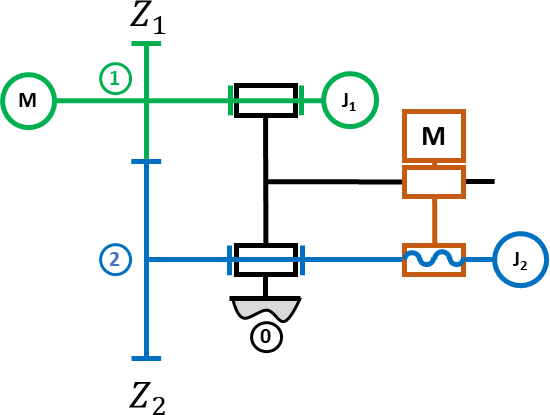
\includegraphics[width=5cm]{fig_07}
\end{center}
\begin{multicols}{4}
	\begin{reponses}	
	\mauvaise{$v = \dfrac{ Z_2  }{ Z_1  p } \omega_{10}$}
	\mauvaise{$v = \dfrac{Z_2 p}{2 Z_1  \pi } \omega_{10}$}
	\mauvaise{$v = \dfrac{2 Z_1 \pi }{ Z_2  p } \omega_{10}$}
	\bonne{$v = \dfrac{Z_1 p}{2 Z_2  \pi } \omega_{10}$}
	\end{reponses}
\end{multicols}
\end{question}\\}

